\problemname{Height Profile}

The cycling classic Amstel Gold Race is held annually in the nearby
Dutch province of Limburg. It features frequent short climbs giving
contestants little time to recover in between.  For instance the last
$42$ kilometres of the race has $8$ steep climbs of average length
roughly $1$ kilometre each.

The \emph{incline grade} for each climb is given in percent. An incline grade of $100\%$ means that for
every $1$ horizontal metre travelled, you also travel $1$ vertical metre upwards. An incline grade of $0\%$
is perfectly flat. In general, an incline grade of $p\%$ has $p / 100$ vertical metres for each
horizontal metre. Note that the incline grade can also be negative.

You know the height of the road at integer horizontal kilometres from the start
of the race, and for simplicity we model the heights as being piecewise-linear in between these
points.  In other words, the incline grade is assumed to be constant between $0$ and $1$ km, and between 
$1$ and $2$ km, and so on.  For example, in Figure~\ref{fig:profile}, the height at the horizontal
distance $2.5$ kilometres is exactly $20$ metres.

\vspace{-2mm}
\begin{figure}[h!]
  \centering
  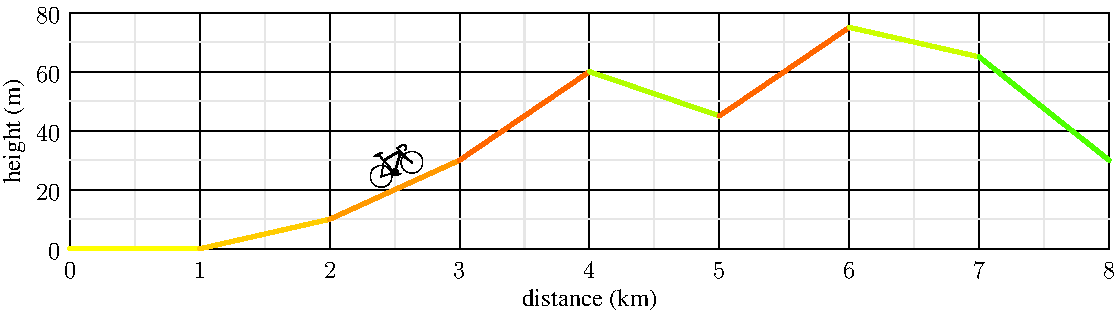
\includegraphics[width=0.9\textwidth]{profile}
  \caption{Illustration of Sample Input 1. The incline grades of the first $3$ horizontal kilometres are
    in order $0\%$, $1\%$ and $2\%$. The last kilometer has an incline grade of $-3.5\%$.}
  \label{fig:profile}
\end{figure}
\vspace{-2mm}

The Amstel Gold Race cannot be compared with some hilly stages of the Tour de France
or the Giro d'Italia, but you are still interested in a comparison. For each one-day race, whether
it is the Amstel Gold Race or one of the stages of the Tour de France, you would like to know the length
of the longest horizontal interval with at least a given incline grade. Actually, you would like
to know the answer for multiple incline grades.

The incline grade of a horizontal interval is measured between the two endpoints. For example, the
incline grade between kilometers $1$ and $4$ of the race in Figure~\ref{fig:profile} is $2\%$, as
$60$ vertical metres are gained in $2$ kilometres. This horizontal interval is also the longest one
with an incline grade of at least $2\%$.

\vspace{-3mm}
\begin{Input}
  The input consists of:
  \begin{itemize}
    \item One line with two integers $n$ and $k$ ($2\leq n\leq 10^5, 1\leq k\leq 50$), the
      horizontal length of the race in kilometres and the number of incline grades you have chosen.
    \item One line with $n + 1$ integers $h_0, h_1, \ldots, h_n$ ($0\leq h_i\leq 10^9$), where
      $h_i$ is the height of the route in metres $i$ horizontal kilometres from the start.
    \item $k$ lines each containing a real number $g$ ($-100 \le g \le 100$ and $g$ has exactly one digit after the decimal point), an incline grade you care about.
  \end{itemize}
\end{Input}

\begin{Output}
  For each of the $k$ given incline grades, in the same order as in the input, output the length in
  kilometres of the longest horizontal interval with at least this incline grade. If no suitable
  interval exists, output ``\texttt{impossible}''.

  Your answers should have an absolute or relative error of at most $10^{-6}$.
\end{Output}
